\pagestyle{plain}
\chapter{Développements Logiciel : Conception, Modélisation, Implémentation} 

\section{Développements logiciel}
Dans le cadre du projet, plusieurs éléments ont été développés, à noter, une intelligence artificielle pour détecter des seiches dans une image, une base de données de seiches pour entraîner l'intelligence artificielle et un algorithme de filtre à particule utilisant des descripteurs et mesures de similarité pour calculer le poids de chaque particule.\\

\subsection{Intelligence Artificielle}
La base de données d'images de seiches est composée d'images provenant de vidéos de seiches prises par des plongeurs en mer, et par des particuliers dans des aquariums.\\
Chaque image a été annotée à la main par les membres du groupe en utilisant le logiciel en ligne Roboflow, la base de données est constituée d'un total de 5175 images.\\
L'intelligence artificielle utilise le code et les poids pré-entrainés de YOLOv7\cite{wang_yolov7_nodate}, qui peuvent être trouvé sur le github officiel de YOLOv7\cite{yolov7_github}.
Cette intelligence artificielle a été entrainée pour 300 cycles de la base de données, soit un total de 25 heures sans interruptions.\\
Les performances obtenues sont illustrées dans la figure \ref{fig:ai_results} et des exemples sont donnés en figure \ref{fig:ai_examples}.\\

\begin{figure}[!htbp]
\center
	\subfloat[Precision]{{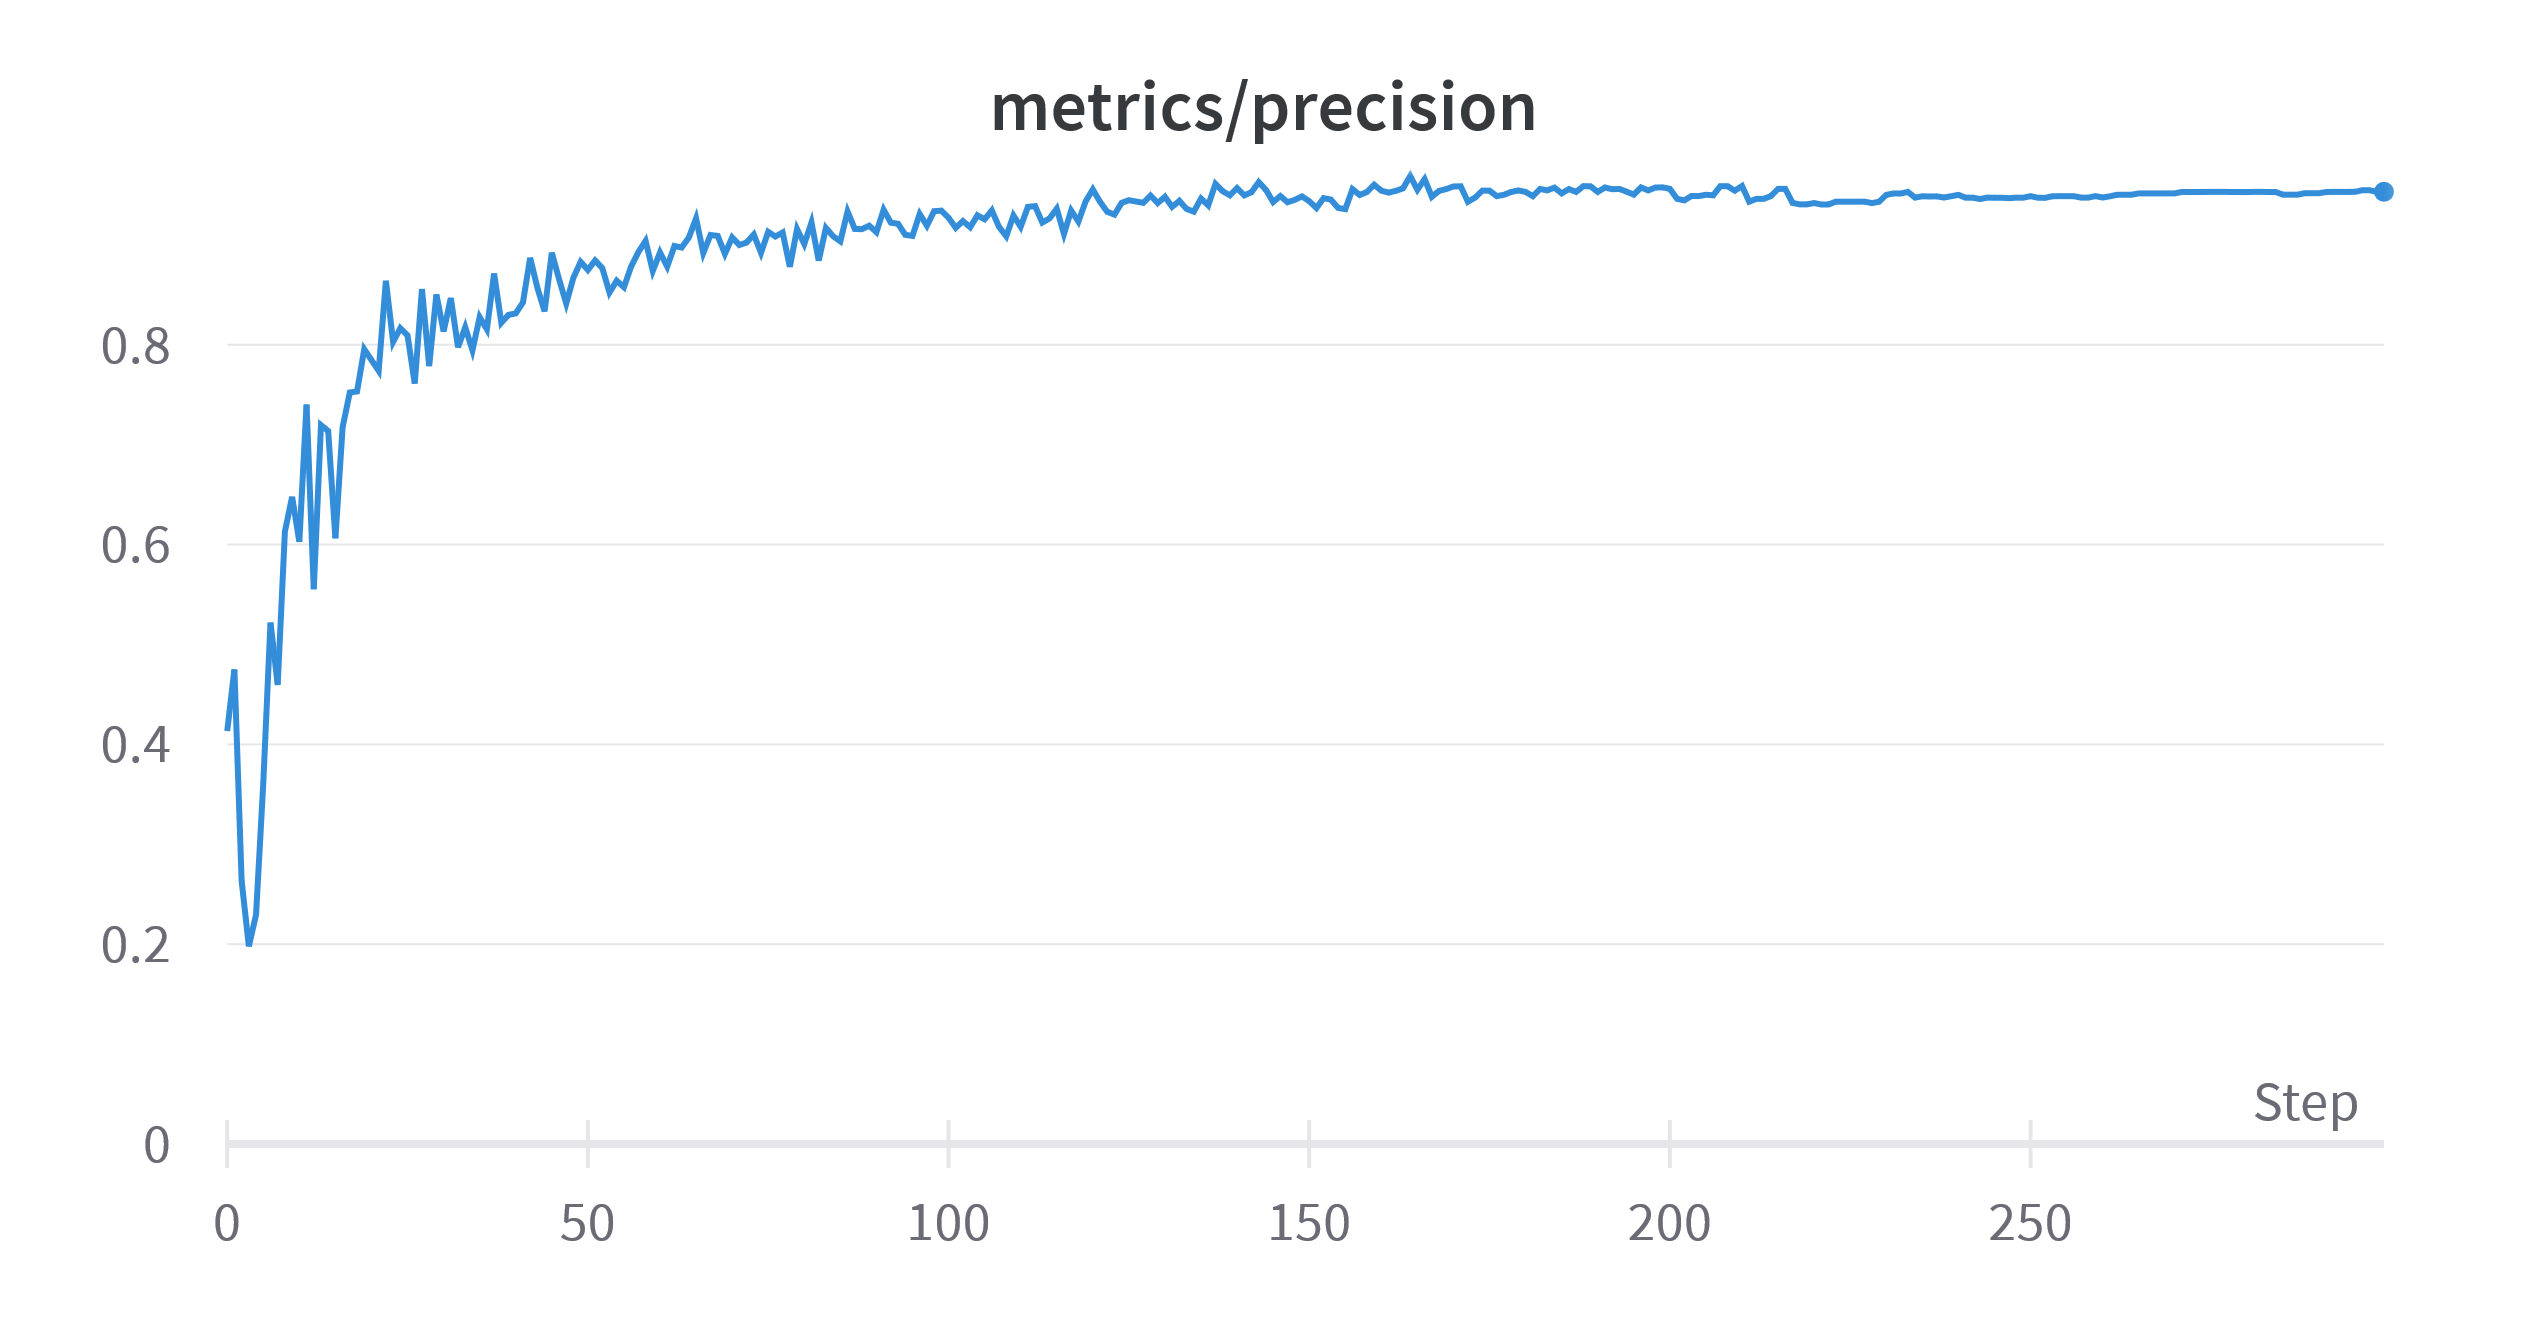
\includegraphics[scale=0.07]{metricsprecision.png}}}
	\subfloat[Recall]{{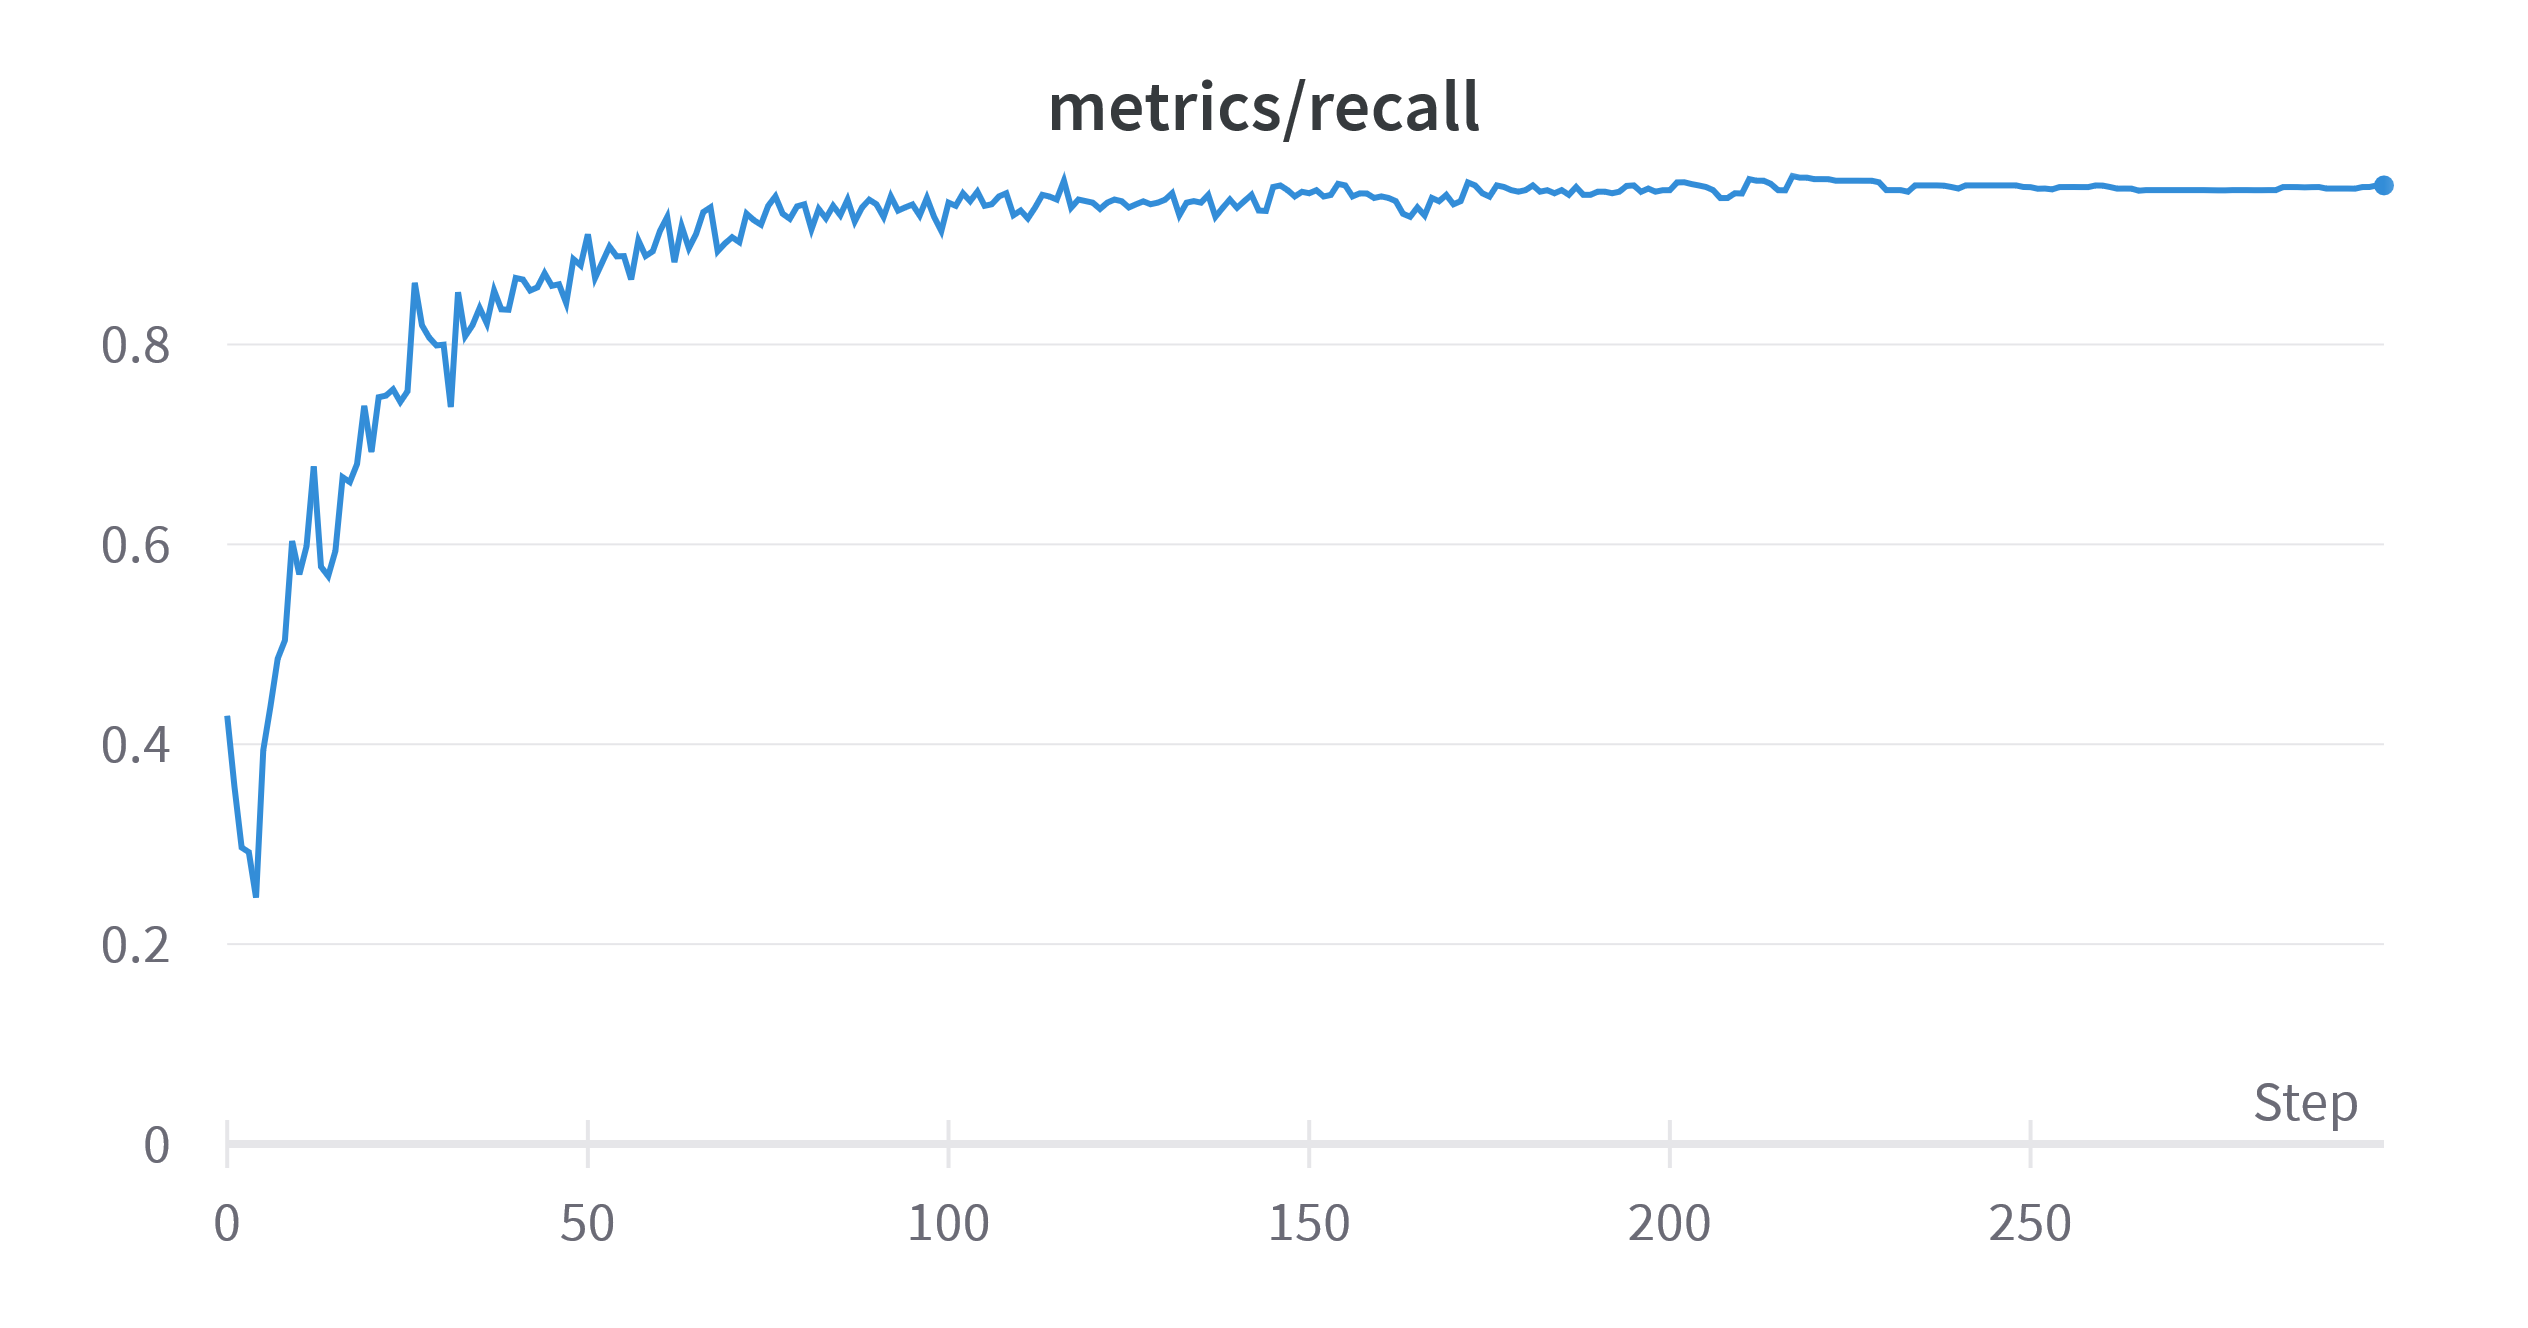
\includegraphics[scale=0.07]{metricsrecall.png}}}
	\\
	\subfloat[mAP@.5]{{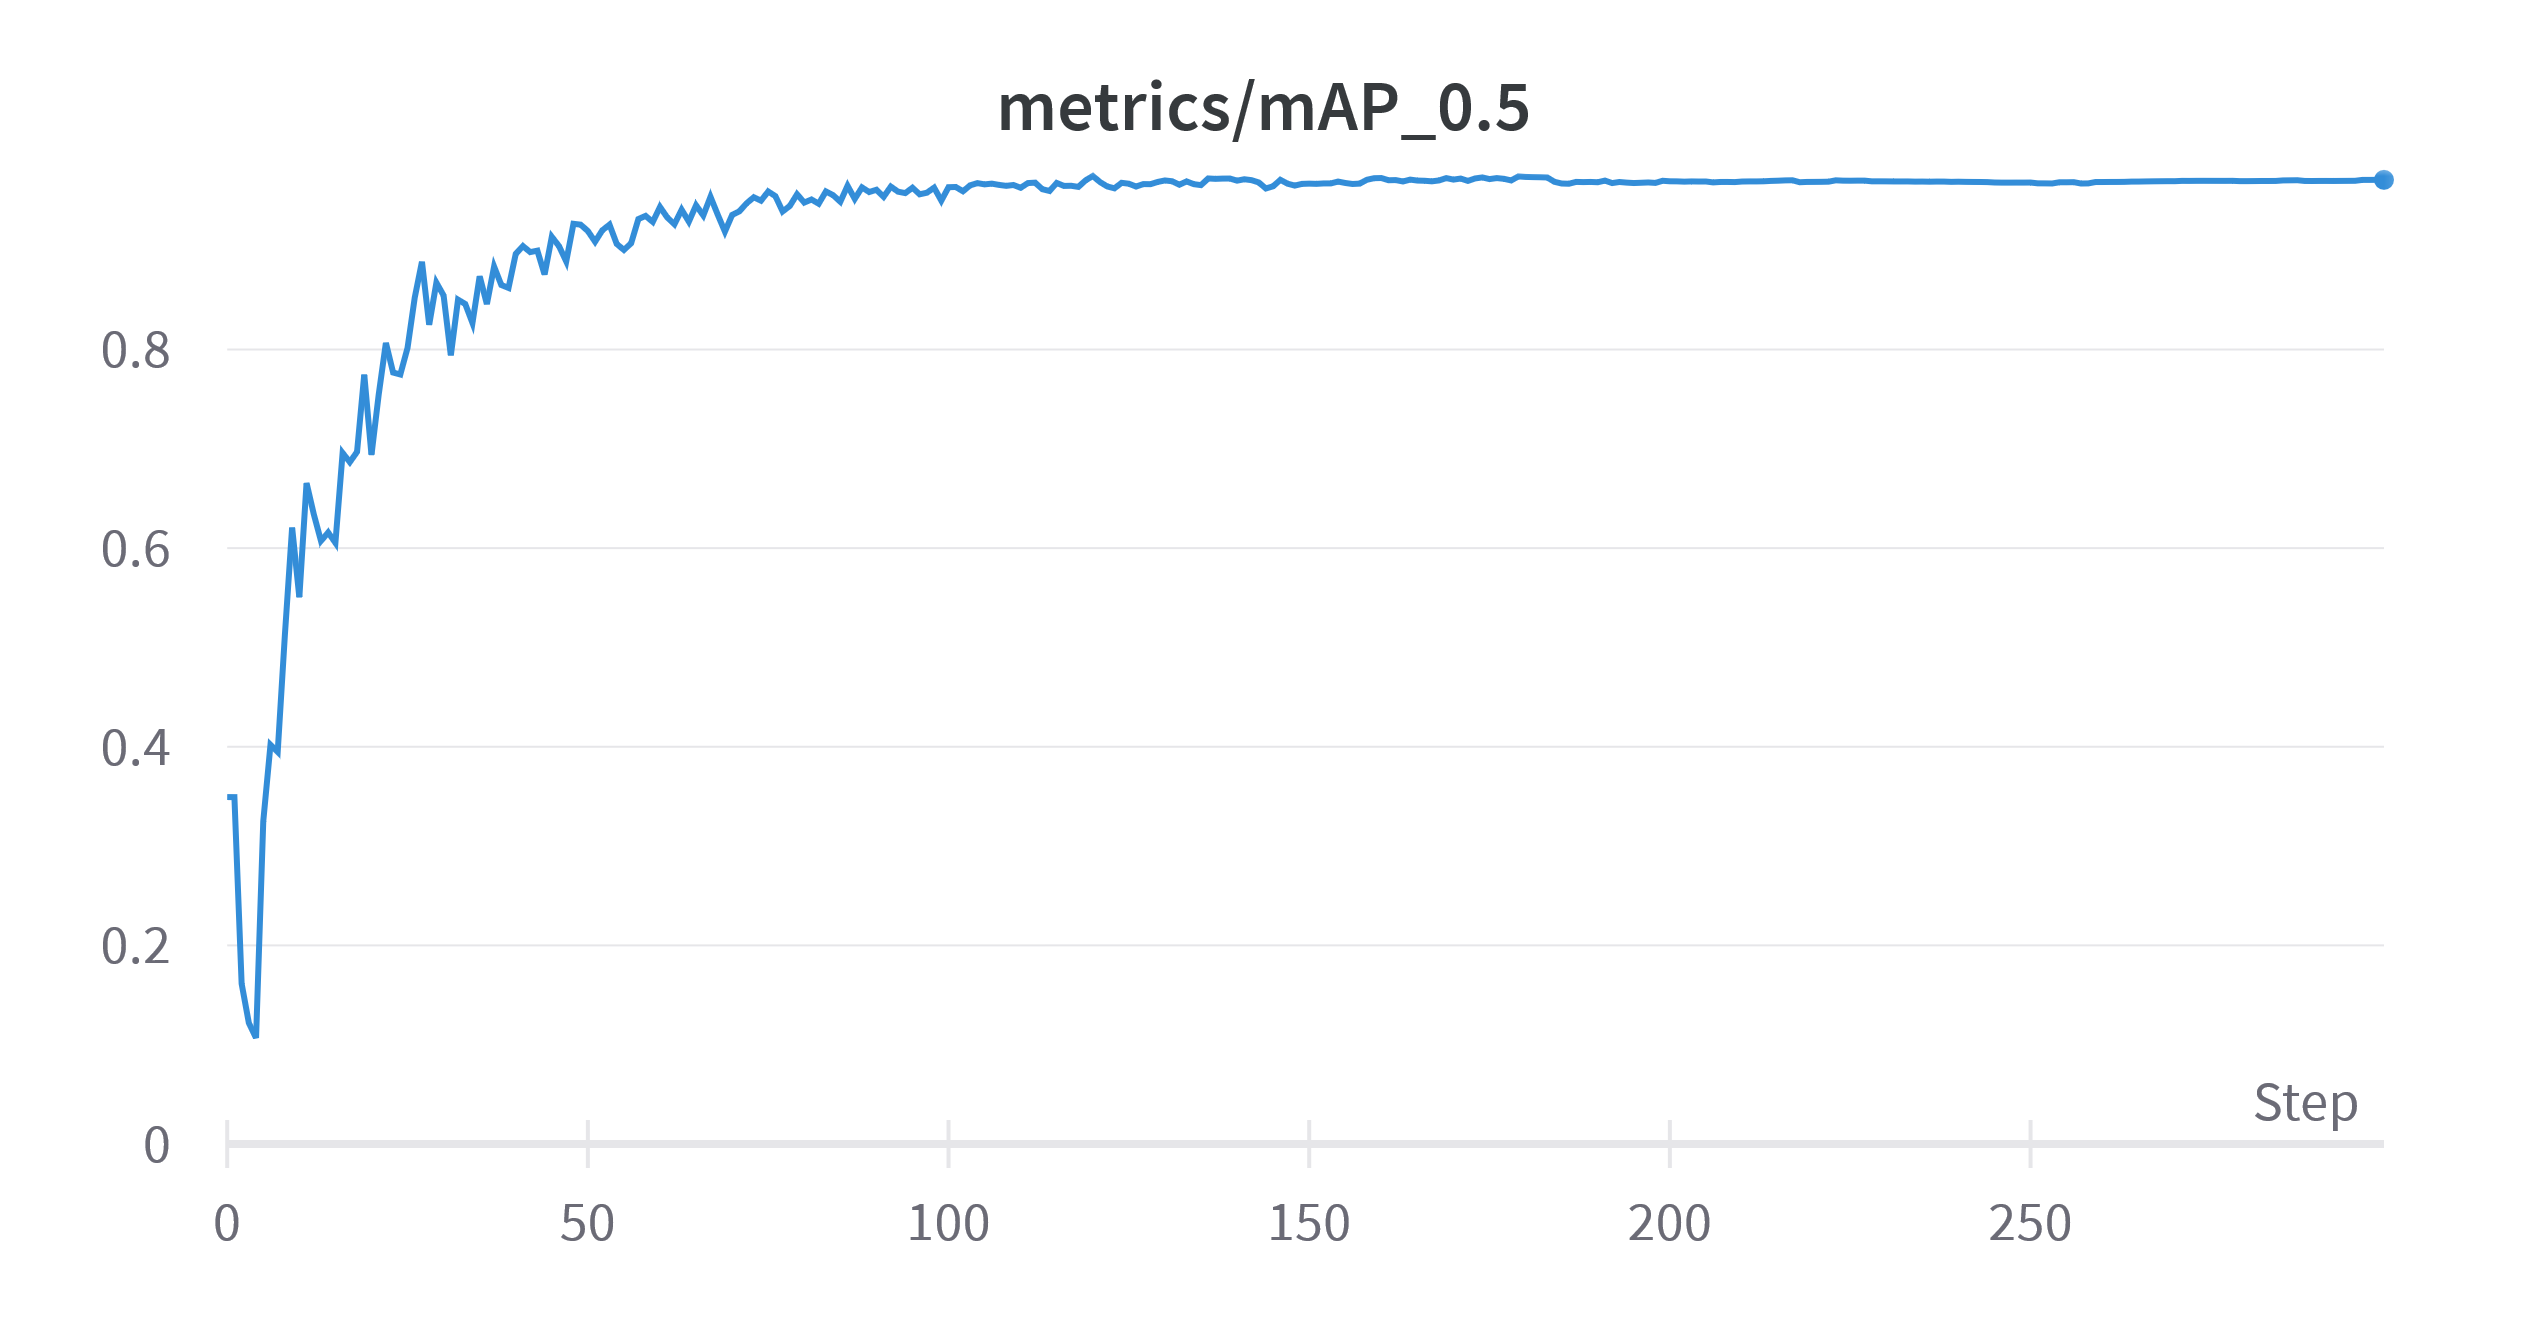
\includegraphics[scale=0.07]{metricsmAP_0.5.png}}}
	\subfloat[mAP@.5:.95]{{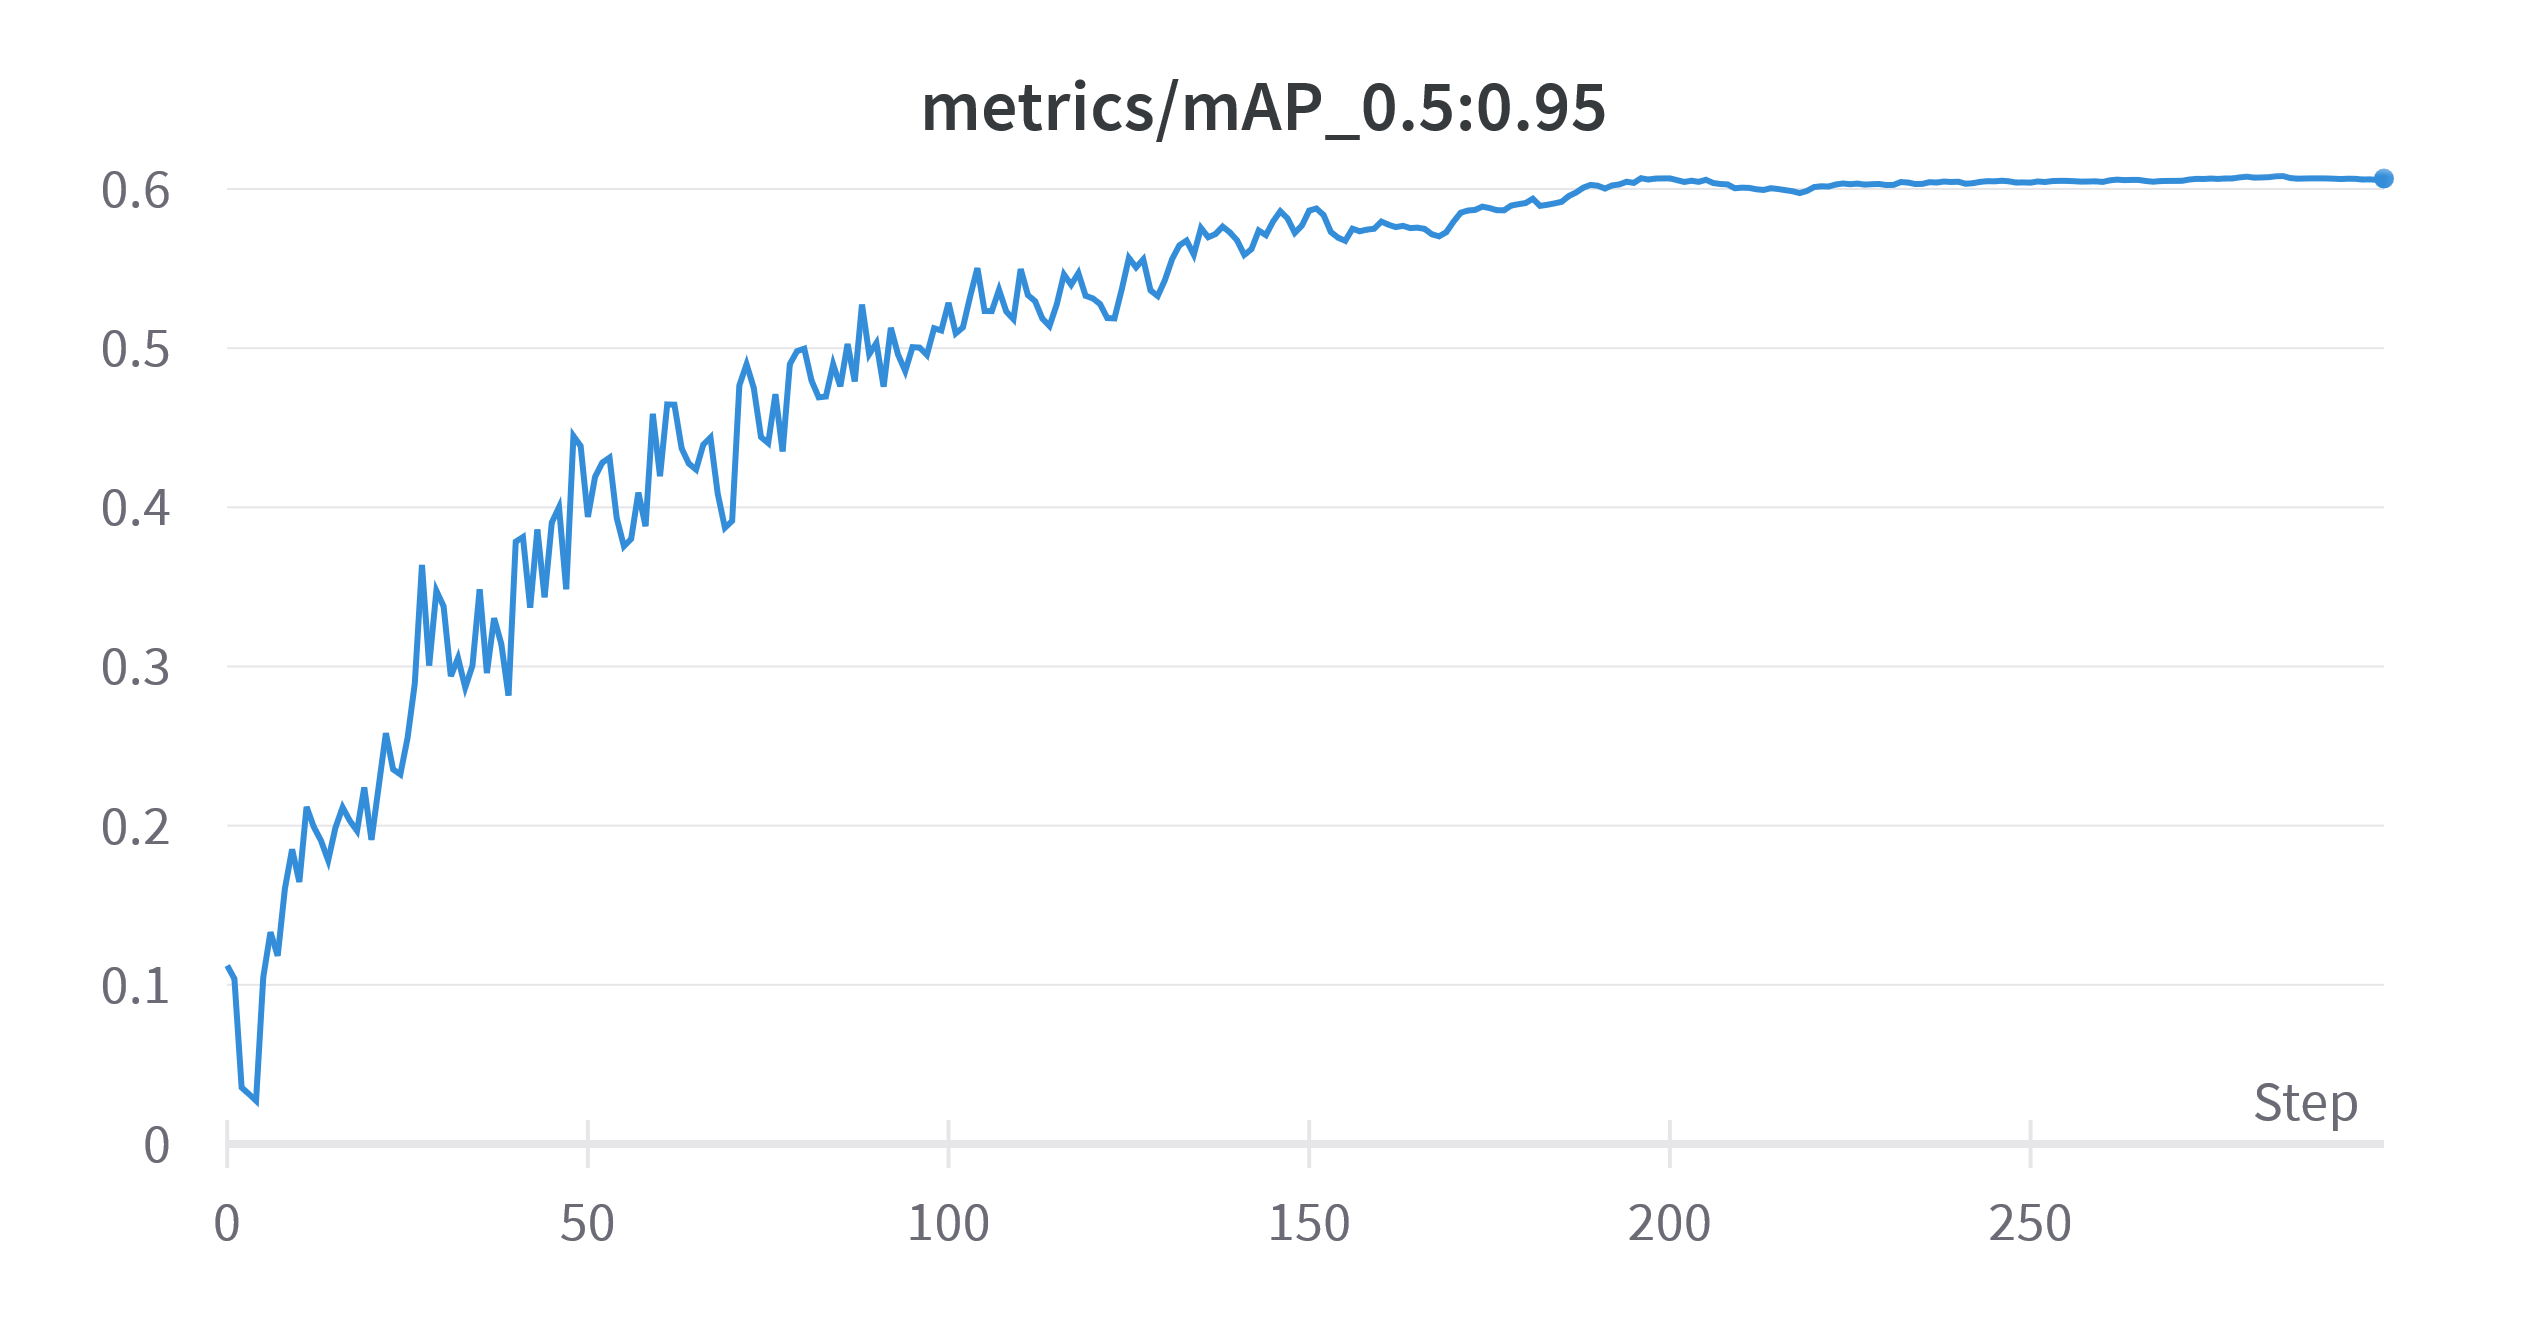
\includegraphics[scale=0.07]{metricsmAP_0.5_0.95.png}}}
\caption{Performances de notre modèle après entrainement.}
\label{fig:ai_results}
\end{figure}
\FloatBarrier

Les différentes définitions peuvent être retrouvées en annexe (\ref{app:mAP}).\\
%Nombre de vrai positif divisé par le nombre de vrai positif plus le nombre de faux positif
%Nombre de vrai positif divisé par le nombre de positif total
\\
Les résultats obtenus sont compilés dans le tableau suivant:\\
\begin{center}
\begin{tabular}{|c|c|c|c|}
	\hline
	Précision & Recall & mAP@.5 & mAP@.5:.95\\
	\hline
	0.953 & 0.959 & 0.971 & 0.607\\
	\hline
\end{tabular}
\end{center}

\begin{figure}[!htbp]
\center
	\subfloat{{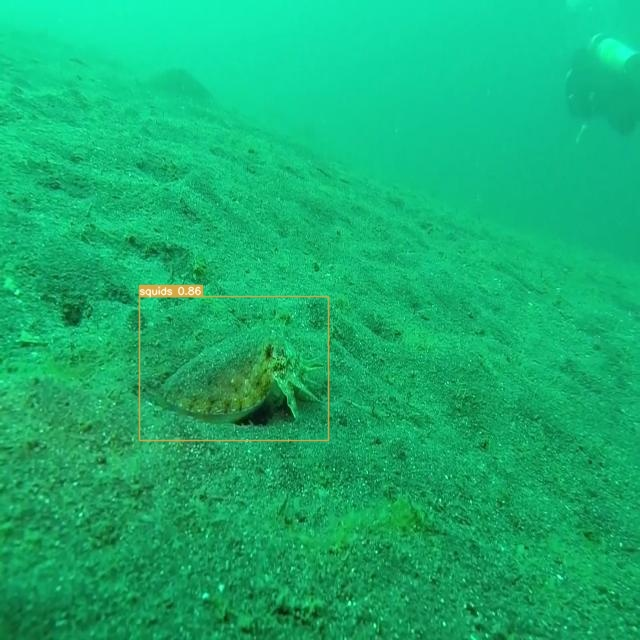
\includegraphics[scale=0.3]{cuttlefish_example1.jpg}}}
	\hspace{0.1cm}
	\subfloat{{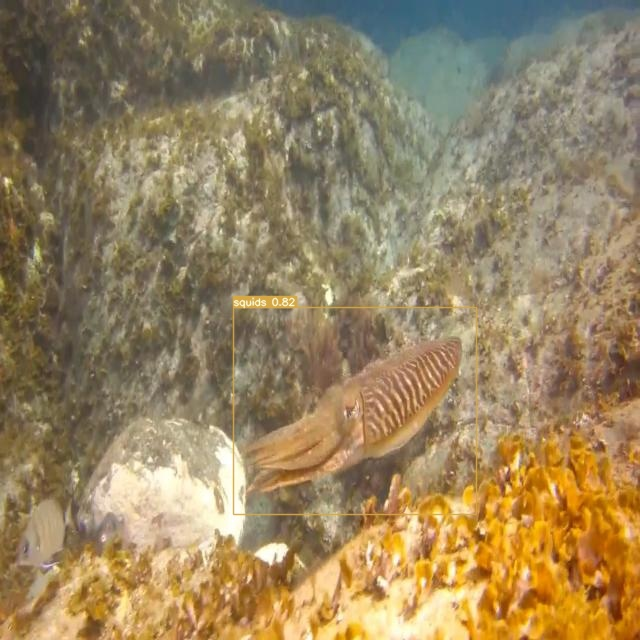
\includegraphics[scale=0.3]{cuttlefish_example2.jpg}}}
	\\
	\subfloat{{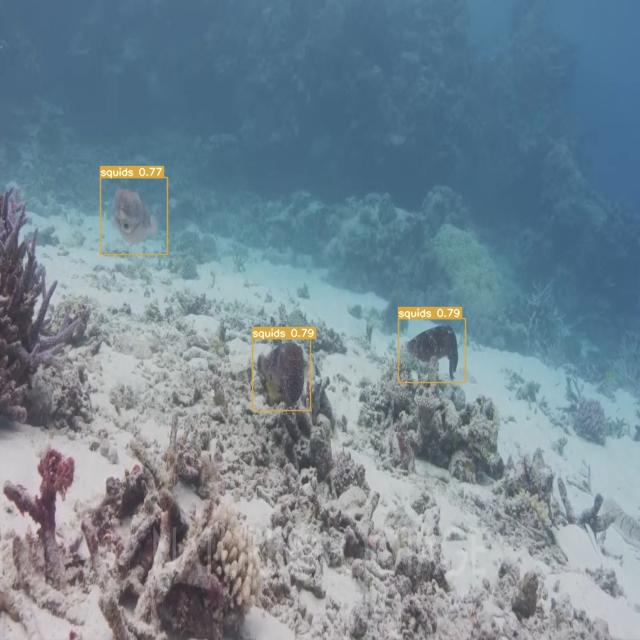
\includegraphics[scale=0.3]{cuttlefish_example3.jpg}}}
	\hspace{0.1cm}
	\subfloat{{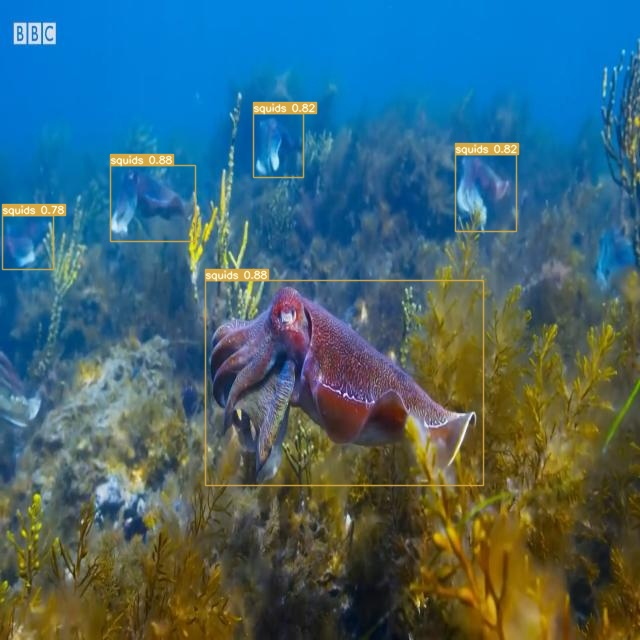
\includegraphics[scale=0.3]{cuttlefish_example4.jpg}}}
\caption{Exemples de résultats obtenus par notre modèle.}
\label{fig:ai_examples}
\end{figure}
\FloatBarrier



\subsection{Logiciel de suivi de seiche}
Ce logiciel est composé d'un filtre à particule, de descripteurs, et de mesures de similarité, qui seront développés en partie \hyperlink{chapter.4}{4}.\\
Il prend en entrée une liste de paramètres pour configurer les différentes parties, et une vidéo. Après configuration du filtre à particule, du descripteur et de la mesure de similarité, la première image de la vidéo est donnée à notre intelligence artificielle, pour avoir une estimation de la position et bounding box d'une seiche que l'on souhaite suivre dans la vidéo.\\
Après le traitement de la première image par notre intelligence artificielle, chaque image de la vidéo est donnée au filtre à particule afin qu'il mette à jour toutes ses particules, et estime au mieux la position et la bounding box de la seiche suivie.\\
Une fois que le filtre à particule a fini de traiter une image, celle-ci est affichée avec la position estimée en bleu et la bounding box estimée en vert, et les meilleures particules en rouge (voir figure \ref{fig:soft_result}). Le numéro de l'image traitée est affiché en haut à gauche de la fenêtre.\\

\begin{figure}[!htbp]
\center
	\subfloat{{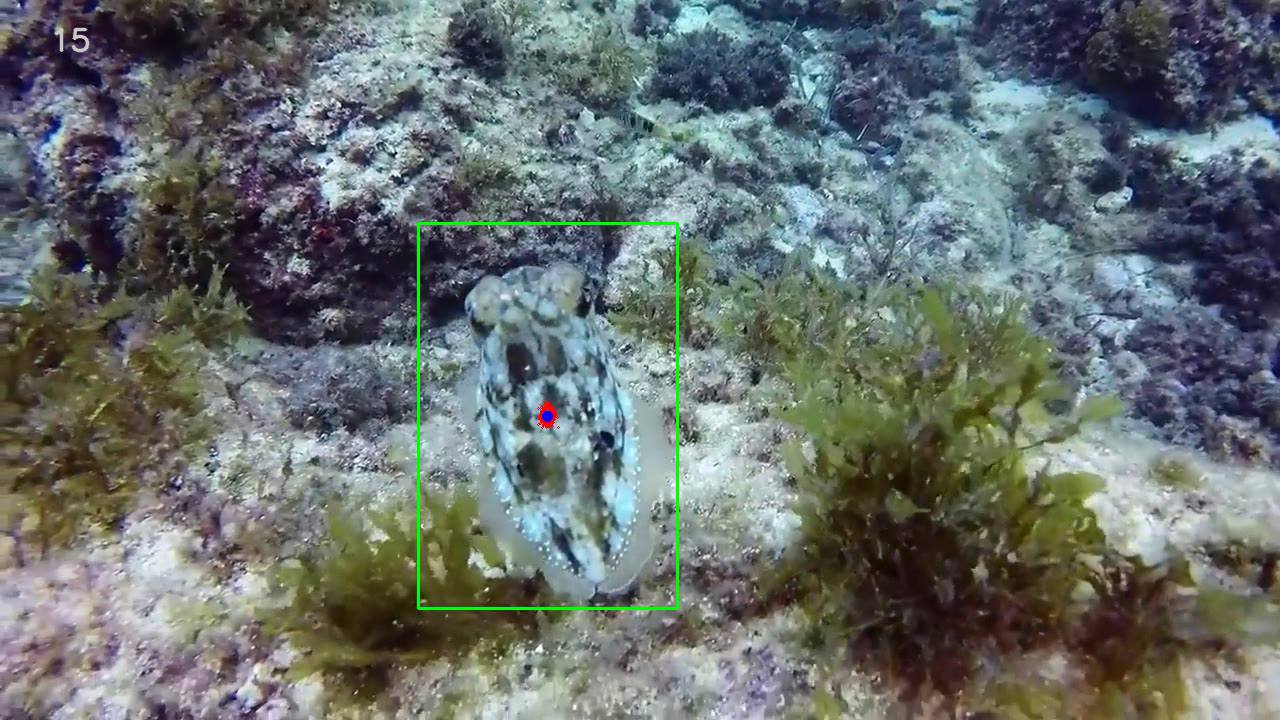
\includegraphics[scale=0.3]{Cuttlefish_results0013.png}}}
\caption{Exemple d'une image renvoyée par le logiciel.}
\label{fig:soft_result}
\end{figure}
\FloatBarrier

Le logiciel donne également la possibilité de sauvegarder la vidéo résultante, ainsi que les valeurs de la particule estimée à chaque itération du filtre.\\
Sauvegarder cette estimation permet, par la suite, d'effectuer une analyse des performances de nos solutions, en utilisant un script d'évaluation qui calcule l'IoU (voir annexe \ref{app:IoU}) entre une estimation à un instant $t$ et la véritable valeur à ce même instant, comme montré dans la figure \ref{fig:eval_result}.\\

\begin{figure}[!htbp]
\center
	\subfloat{{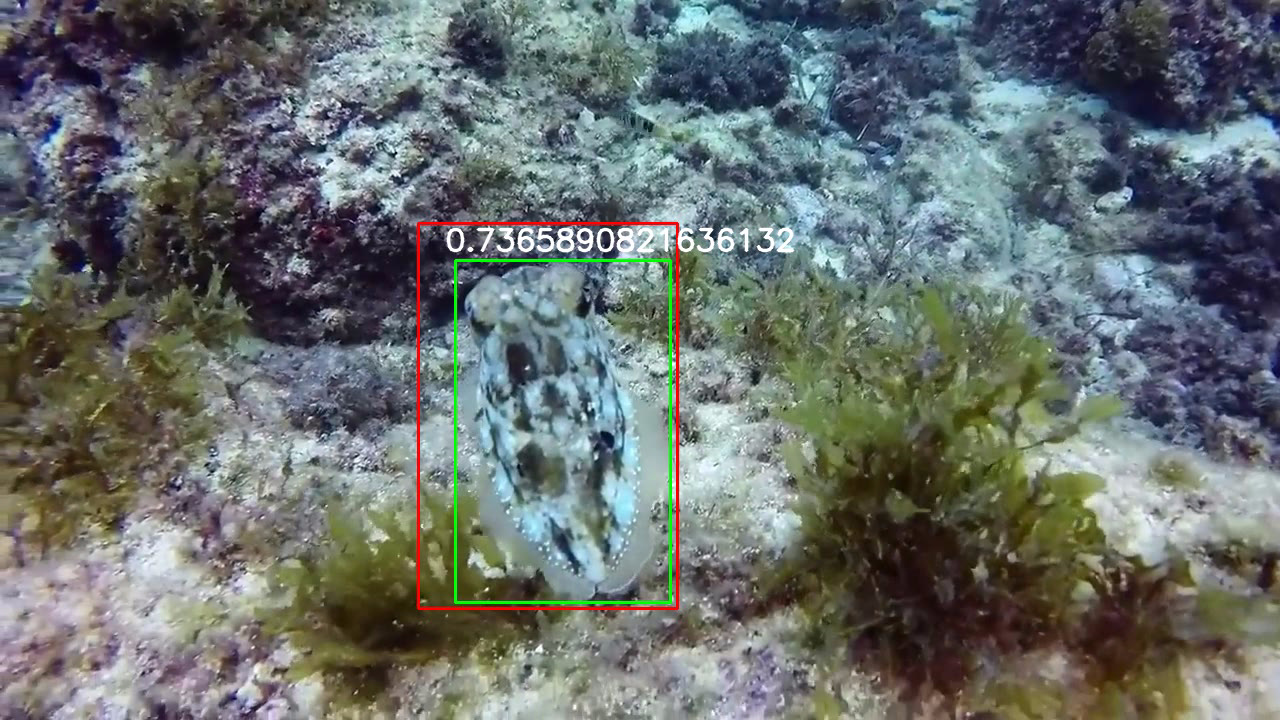
\includegraphics[scale=0.3]{eval0014.png}}}
\caption{IoU (blanc) entre l'image de référence (vert) et notre résultat (rouge).}
\label{fig:eval_result}
\end{figure}
\FloatBarrier


\clearpage
\section{Modules}
Le diagramme UML de cas d'utilisation (figure \ref{fig:uml_diagram_usecase}) du projet est assez simple, et se résume à une unique relation entre l'utilisateur et le logiciel, celle de lancer le programme avec une vidéo et les paramètres souhaités. Le reste des relations est effectué en interne et aucune interaction externe n'est requise.\\
Le diagramme UML global des classes peut être retrouvé en annexe \ref{app:UMLGlobal}.

\begin{figure}[!htbp]
\center
	\subfloat{{
\includegraphics[scale=0.4]{usecase.png}}}
\caption{Diagramme UML de cas d'utilisation.}
\label{fig:uml_diagram_usecase}
\end{figure}
\FloatBarrier


\subsection{Descripteurs}
Le module descripteur est constitué d'une classe parent $Descriptor$ qui possède 5 classes filles, $HOG$, $HOGCASCADE$, $HOGCOLOR$, $LBP$ et $HOGCASCADELBP$. Ces classes sont les différents descripteurs que l'utilisateur peut utiliser dans le filtre à particule.\\
Toutes ces classes possèdent deux méthodes communes, la méthode $update$ qui permet de mettre à jour certains paramètres du descripteur, et la méthode $compute$ qui permet d'effectuer le calcul du descripteur sur une liste d'images.\\
A noter, que les descripteurs $HOGCASCADE$ et $HOGCOLOR$ sont des variantes du descripteur $HOG$ (HOG et HOG cascade seront détaillés en partie \hyperlink{chapter.4}{4}), et le descripteur $HOGCASCADELBP$ est une combinaison entre un descripteur HOG cascade et LBP.\\
\\
Ce module permet de calculer, pour chaque particule du filtre, un vecteur descripteur qui pourra, par la suite, être comparé avec un descripteur de référence pour estimer la similarité entre la particule et une particule de référence.\\
Le diagramme UML du module est donné en figure \ref{fig:uml_diagram_descriptor}.

\begin{figure}[!htbp]
\center
	\subfloat{{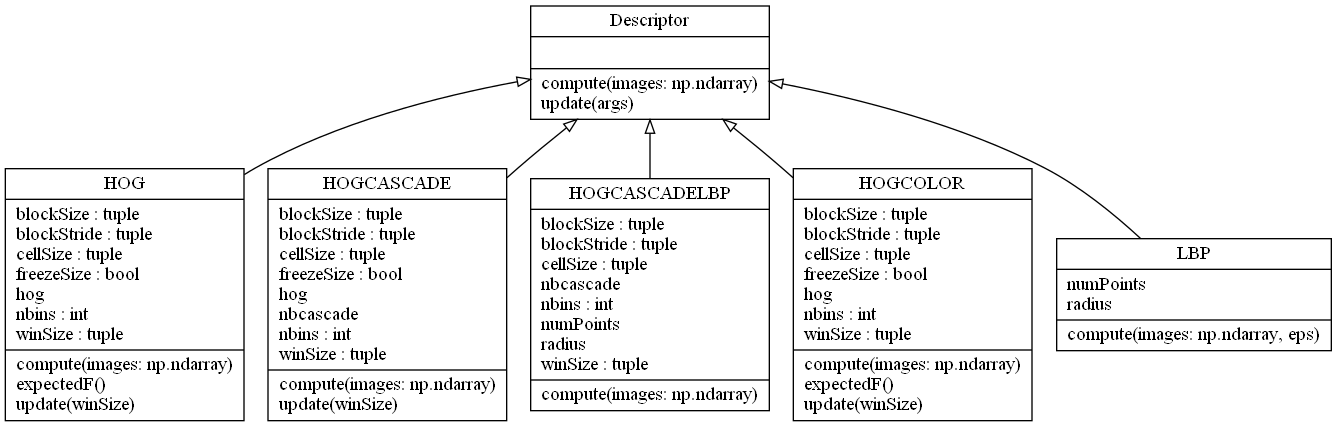
\includegraphics[scale=0.4]{descriptors.png}}}
\caption{Diagramme UML des classes du module descripteur.}
\label{fig:uml_diagram_descriptor}
\end{figure}
\FloatBarrier




\subsection{Mesure de similarité}
Le module mesure de similarité est constitué d'une classe parent $Similarity$ qui possède 4 classes filles, $Bhattacharyya\_sqrt$, $Bhattacharyya\_log$, $Cosine\_Similarity$ et $Kullback\_Leibler\_Divergence$. Ces classes sont les différentes mesures de similarité que l'utilisateur peut utiliser dans le filtre à particule.\\
Toutes ces classes possèdent une méthode commune, la méthode $computeSimilarity$ qui permet de calculer la similarité entre une liste de vecteurs descripteur et un vecteur descripteur de référence.\\
Les mesures de similarité $Bhattacharyya\_sqrt$ et $Cosine\_Similarity$ seront détaillées en partie \hyperlink{chapter.4}{4}.\\
\\
Ce module permet de calculer, pour chaque descripteur de chaque particule du filtre, un coefficient de similarité qui indique quelles particules sont les plus probables de représenter la position de la seiche à un instant $t$.\\
Le diagramme UML du module est donné en figure \ref{fig:uml_diagram_similarity}.

\begin{figure}[!htbp]
\center
	\subfloat{{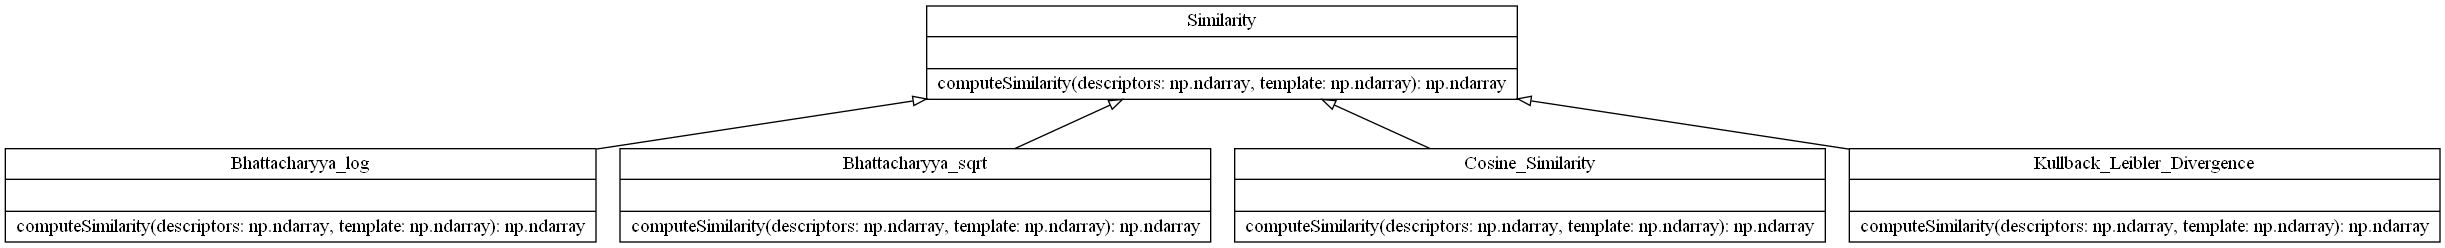
\includegraphics[scale=0.2]{similarity.png}}}
\caption{Diagramme UML des classes du module mesure de similarité.}
\label{fig:uml_diagram_similarity}
\end{figure}
\FloatBarrier




\subsection{Filtre à particule}
Le module filtre à particule est le plus conséquent, car il regroupe plusieurs autres modules, comme les modules descripteur et mesure de similarité. La classe $ParticleFilter$ est la classe principale de ce module et implémente l'algorithme du filtre à particule. Elle fait appel aux classes $Particle$, $Descriptor$, $Slicer$, $Resampling$ et $Similarity$, et les utilise ensemble pour effectuer le suivi d'une seiche.\\
\\
Ce module est responsable de fournir tous les résultats nécessaires au programme principal, pour qu'il puisse les afficher et/ou les sauvegarder pour être finalement évalués. Ce module est très flexible et permet d'être configuré avec différentes structures de particules, différents descripteurs, différentes mesures de similarité, ou encore différentes méthodes de ré-échantillonnage.\\
Le diagramme UML du module est donné en figure \ref{fig:uml_diagram_particlefilter}.

\begin{figure}[!htbp]
\center
	\subfloat{{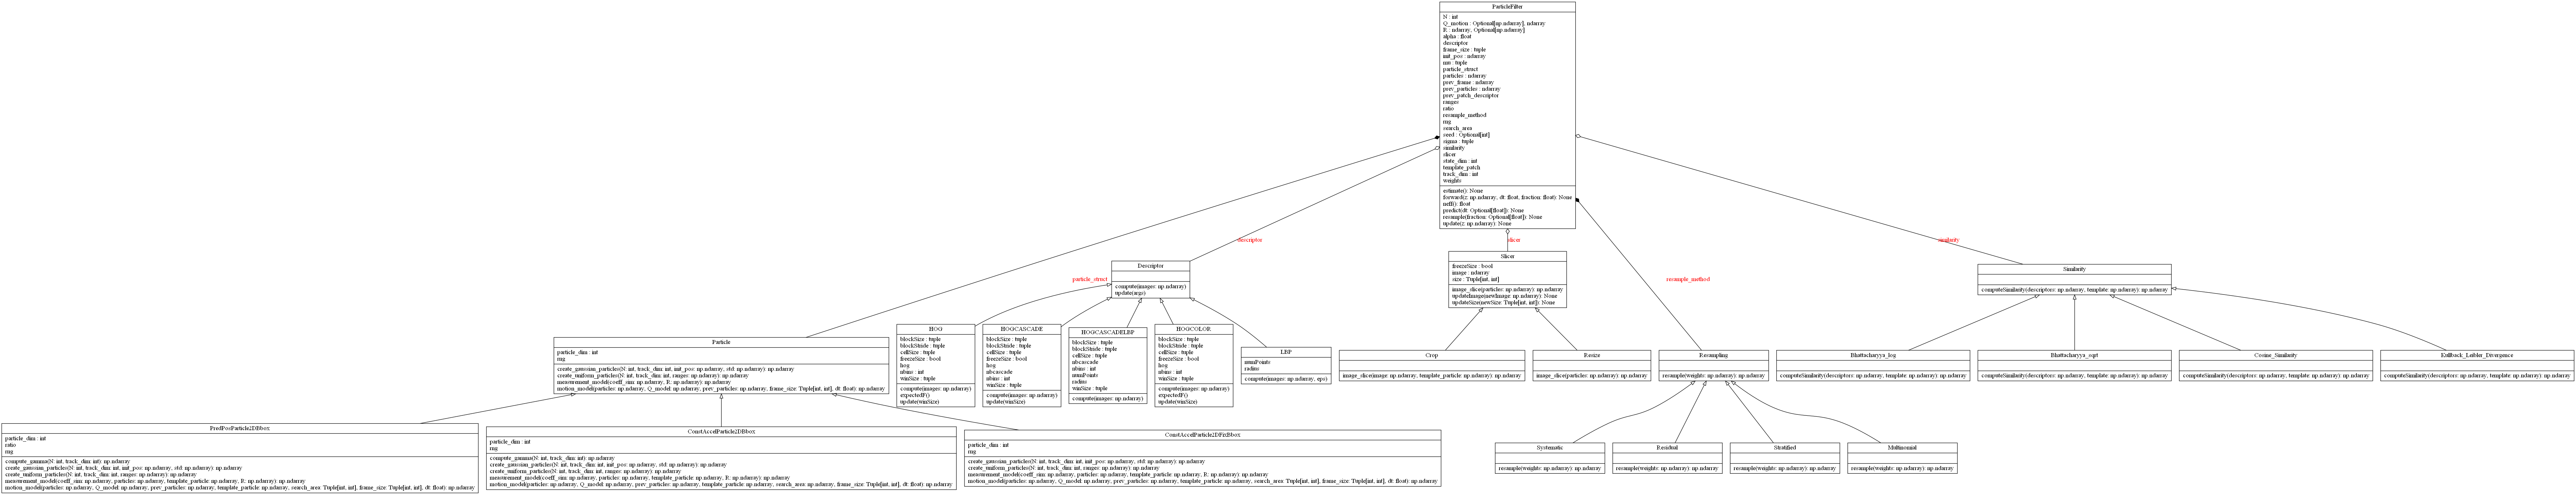
\includegraphics[scale=0.065]{particlefilter.png}}}
\caption{Diagramme UML des classes du module filtre à particule.}
\label{fig:uml_diagram_particlefilter}
\end{figure}
\FloatBarrier





\section{Structures de données}
Les structures de données principales du projet sont les tenseurs en tant que tableaux multidimensionnels, pour ce faire, nous utilisons la librairie Numpy, qui permet de réaliser des opérations sur ces tableaux de façon optimisée.\\
Nous essayons de garder les données un maximum sous ce format, pour éviter les conversions et opérations qui pourraient ralentir le logiciel de suivi. C'est pour cela que la majorité des entrées des programmes réalisés demande des 'ndarray', qui est le type des tableaux Numpy.\\
\\
Les images prises en entrée des programmes sont transformées en tableau Numpy, selon la convention de OpenCV, c'est-à-dire avec les couleurs au format BGR et la hauteur de l'image comme première dimension du tenseur, et la largeur de l'image comme seconde dimension.\\
\\
L'utilisateur du logiciel n'intervient qu'à un seul niveau dans le programme, le reste des entrées du logiciel est géré en interne afin de préserver au mieux l'intégrité des données traitées.\\
L'utilisateur peut uniquement donner des paramètres au logiciel lorsqu'il le lance, ces paramètres sont alors parsés en différent arguments qui sont vérifiés par le programme, puis utilisés pour initialiser les différents modules, afin de commencer le suivi d'une seiche.




\section{Statistiques}
Le projet compte un total de 25 classes réparties dans 10 scripts python (voir figure \ref{fig:uml_diagram_classes} en annexe).\\
Les scripts et classes de YOLOv7\cite{wang_yolov7_nodate} utilisés dans le projet ne sont pas comptés.\\
Le projet compte en tout 1587 lignes de code.\\
L'entièreté du projet est en accès libre sur github (\cite{pp2pf}).

\clearpage
